\documentclass[11pt]{article}
\usepackage{anysize,comment,tcolorbox,multicol,enumitem}
\usepackage{HW}
\usepackage{graphics}
\usepackage{float}

\includecomment{comment}
% \excludecomment{studentSpace}
\includecomment{studentSpace}

\includecomment{answer}
\excludecomment{answer}
\includecomment{comment}
\newcommand{\blank}{
\underline{\hspace{1.5cm}\hspace{1.5cm}}
}
\newcommand{\norm}[1]{\left\lVert#1\right\rVert}

\begin{document}
\titleline{\student}
\exhead{Task 03: Announced 29/01. Due: 10:00 PM,  04-Feb}

\begin{enumerate}

%%%%% Question 1
\begin{tcolorbox}
\item  State whether or not the following points are the same and explain why.
\begin{multicols}{2}
\begin{enumerate}[]
\item
$A[2, -1, 3]$, $B[4,-2,6]$
\item
$A[\sqrt{2}/2, -1,0]$, $B[1,-\sqrt{2},0]$
\end{enumerate}
\end{multicols}

\begin{studentSpace}
{\color{blue} In order to compare the above homogeneous points, we need to see if they are linearly dependent or not.

a) $A[2, -1, 3]$,  $B[4,-2,6]$\\
\indent{$\alpha*([2,-1,3]) = [4,-2,6]$ for $\alpha = 2$. Thus, the points are the same.}


b) $A[\sqrt{2}/2, -1,0]$, $B[1,-\sqrt{2},0]$\\
\indent $\alpha*([\sqrt{2}/2, -1,0]) = [1,-\sqrt{2},0]$ for $\alpha = \sqrt{2}$. Thus, the points are the same.
}
% \vspace{3cm}
\end{studentSpace}

%%%%% Question 2
\end{tcolorbox} \begin{tcolorbox}
\item In projective three-space, what are the standard homogeneous
  coordinates of (a) the origin and (b) ideal points determined by the
  intersections of the extensions of the coordinate axes and the ideal
  plane?\\


\begin{studentSpace}
% \vspace{3cm}
{\color{blue} 
Origin: $[0,0,0,1]$ \\
Ideal Points: The ideal plane is represented by $w=1$ plane in $P^{3}$ (assuming homogeneous coordinates in $P^{3}$ are represented by $[x,y,z,w]$). The points of intersection of the coordinate axes with the ideal plane are the following: \\
x-intercept: $[1,0,0,0]$\\
y-intercept: $[0,1,0,0]$\\
z-intercept: $[0,0,1,0]$

}
\end{studentSpace}
\end{tcolorbox}

%%%%% Question 3
\begin{tcolorbox}
\item Write standard homogeneous coordinates for the points specified
  in uppercase characters. (Use left and right to distinguish.)\\

\begin{studentSpace}
% \vspace{3cm}
 {\color{blue}
  \textbf{Left Points:} $A$ = $[-1.5,1]$, $B$ = $[3,1]$, $C$ = $[5,1]$, $D$ = $[5.5,1]$, $E$ = $[1,0]$\\
  \textbf{Right Points:} $A$ = $[0,0,1]$ , $B = [2,0,1]$, $C = [3,1,1]$, $D = [4.5, 5, 0]$ \\
  $E$ = $[-1, 4.5, 1]$, $F$ = $[-4,5,0]$ , $G$ = $[-3,4,1]$, $H$ = $[-4,3,1]$\\
  $I$ = $[-1,1,1]$ , $J$ = $[-4,-2,1]$, $K$ = $[1,-4,1]$, $L$ = $[1.5, -0.5, 1]$\\
  $M$ = $[1,0,0]$
 }
\end{studentSpace}
\end{tcolorbox} 

%%%%% Question 4
\begin{tcolorbox}
\item Which of the following points lie on the line $3p_1 -2p_2+5p_3 =
  0$?  Why?\\
\begin{multicols}{2}
\begin{enumerate}[]
\item
$A[1,1,2]$
\item
$B[4,1,-2]$
\end{enumerate}
\end{multicols}
\begin{studentSpace}
% \vspace{3cm}
{\color{blue}
 Points lie on the line when the homogeneous coordinates satisfy the line's equation.\\
 a) $A[1,1,2]$\\
    Substituting $A$ in equation $3p_1 -2p_2+5p_3 = 0 \Rightarrow 3(1) - 2(1) + 5(2) \neq 0$\\
    thus, $A$ doesn't lie on the line.\\
 a) $B[4,1,-2]$\\
    Substituting $B$ in equation $3p_1 -2p_2+5p_3 = 0 \Rightarrow 3(4) - 2(1) + 5(-2) = 0$ \\
    thus, $B$ lies on the line.\\
}
\end{studentSpace}
\end{tcolorbox} 


%%%%% Question 5
\begin{tcolorbox}
\item Write the coordinates of the lines that are the extensions to the
  projective plane of the following Euclidean lines.
\begin{multicols}{2}
\begin{enumerate}[]
\item
$3x + 2y = 6$
\item
$4x + 5y + 7 = 0$
\end{enumerate}
\end{multicols}
\begin{studentSpace}
% \vspace{3cm}
{\color{blue}
Euclidean lines correspond to planes in the $P^{2}$ projective space. Thus the equation of a line can be treated as that of a plane, taking the $z$ coordinate = 1.\\
a) $3x + 2y = 6$\\
Corresponding line = $[3,2,-6]$\\

b) $4x + 5y + 7 = 0$\\
Corresponding line = $[4,5,7]$
}
\end{studentSpace}

%%%%% Question 6
\end{tcolorbox} \begin{tcolorbox}
\item Sketch each line in the projective plane whose equation is given
\begin{multicols}{2}
\begin{enumerate}[]
\item
$2p_1 + 3p_2 + 5p_3 = 0$
\item
$3p_1 - 2p_2 - p_3 = 0$
\end{enumerate}
\end{multicols}
\begin{studentSpace}
% \vspace{6cm} (Doubt)
\begin{figure}[H]
    \centering
    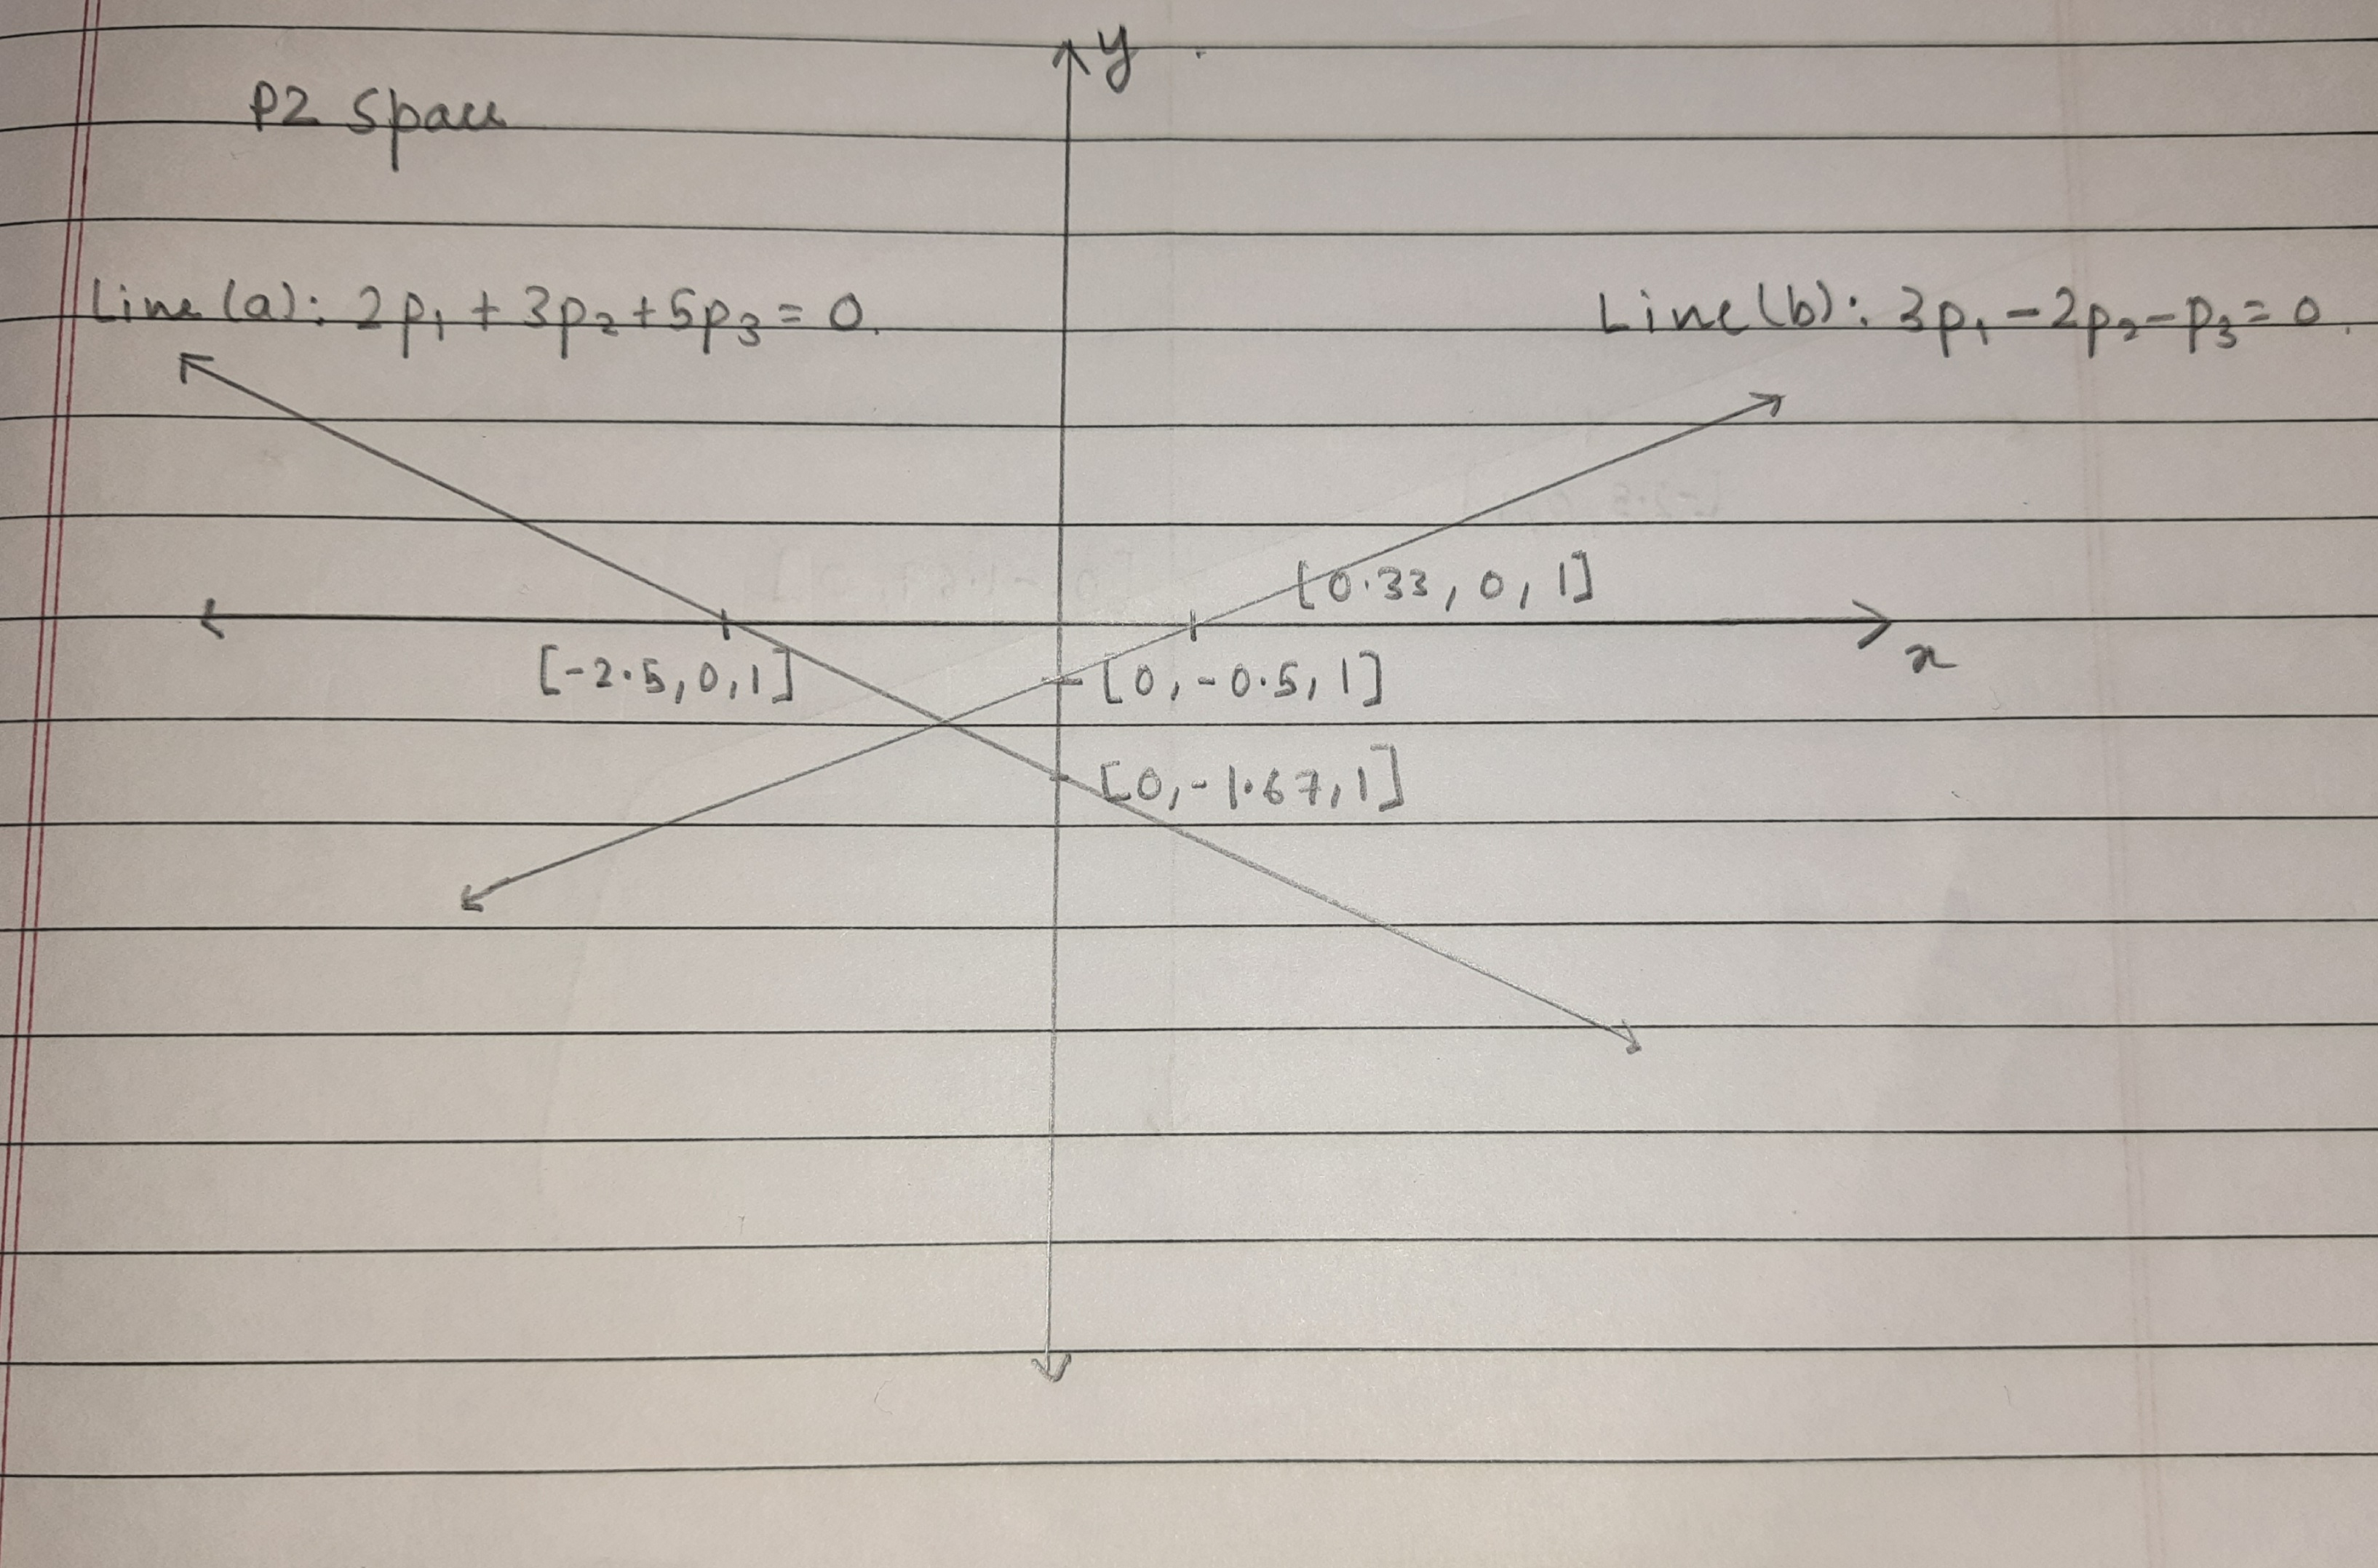
\includegraphics[width = \textwidth, height = 8cm]{01.jpg}
    \caption{{\color{blue} Figure showing the lines (a) and (b)}}
    \label{fig:my_label}
\end{figure}
\end{studentSpace}
\end{tcolorbox}

%%%%% Question 7
\begin{tcolorbox}
\item  In each of the following cases, sketch the line determined by the two given points; then find the equation of the line.
\begin{multicols}{2}
\begin{enumerate}[]
\item
$A[3, 1, 2]$, $B[1,2,-1]$
\item
$A[2,1,3]$, $B[1,2,0]$
\end{enumerate}
\end{multicols}
\begin{studentSpace}
{\color{blue}
Lines are obtained through intersection of two points in the projective space that can be found through the cross product of their homogenous coordinates.\\

a)$AB$ = $[A \times B]$ \Rightarrow $[3,1,2] \times [1,2,-1]$ = $[-5, 5, 5]$ which is equivalent to $[-1,1,1]$

b)$AB$ = $[A \times B]$ \Rightarrow $[2,1,3] \times [1,2,0]$ = $[-6, 3, 3]$ which is equivalent to $[-2,1,1]$\\
Also, note that B is an ideal point, thus to find the line equation, we extend B till we find it on $L_{\infty}$, and the we draw a line between that point (say $B'$) and $A$.
}
\begin{figure}[H]
    \centering
    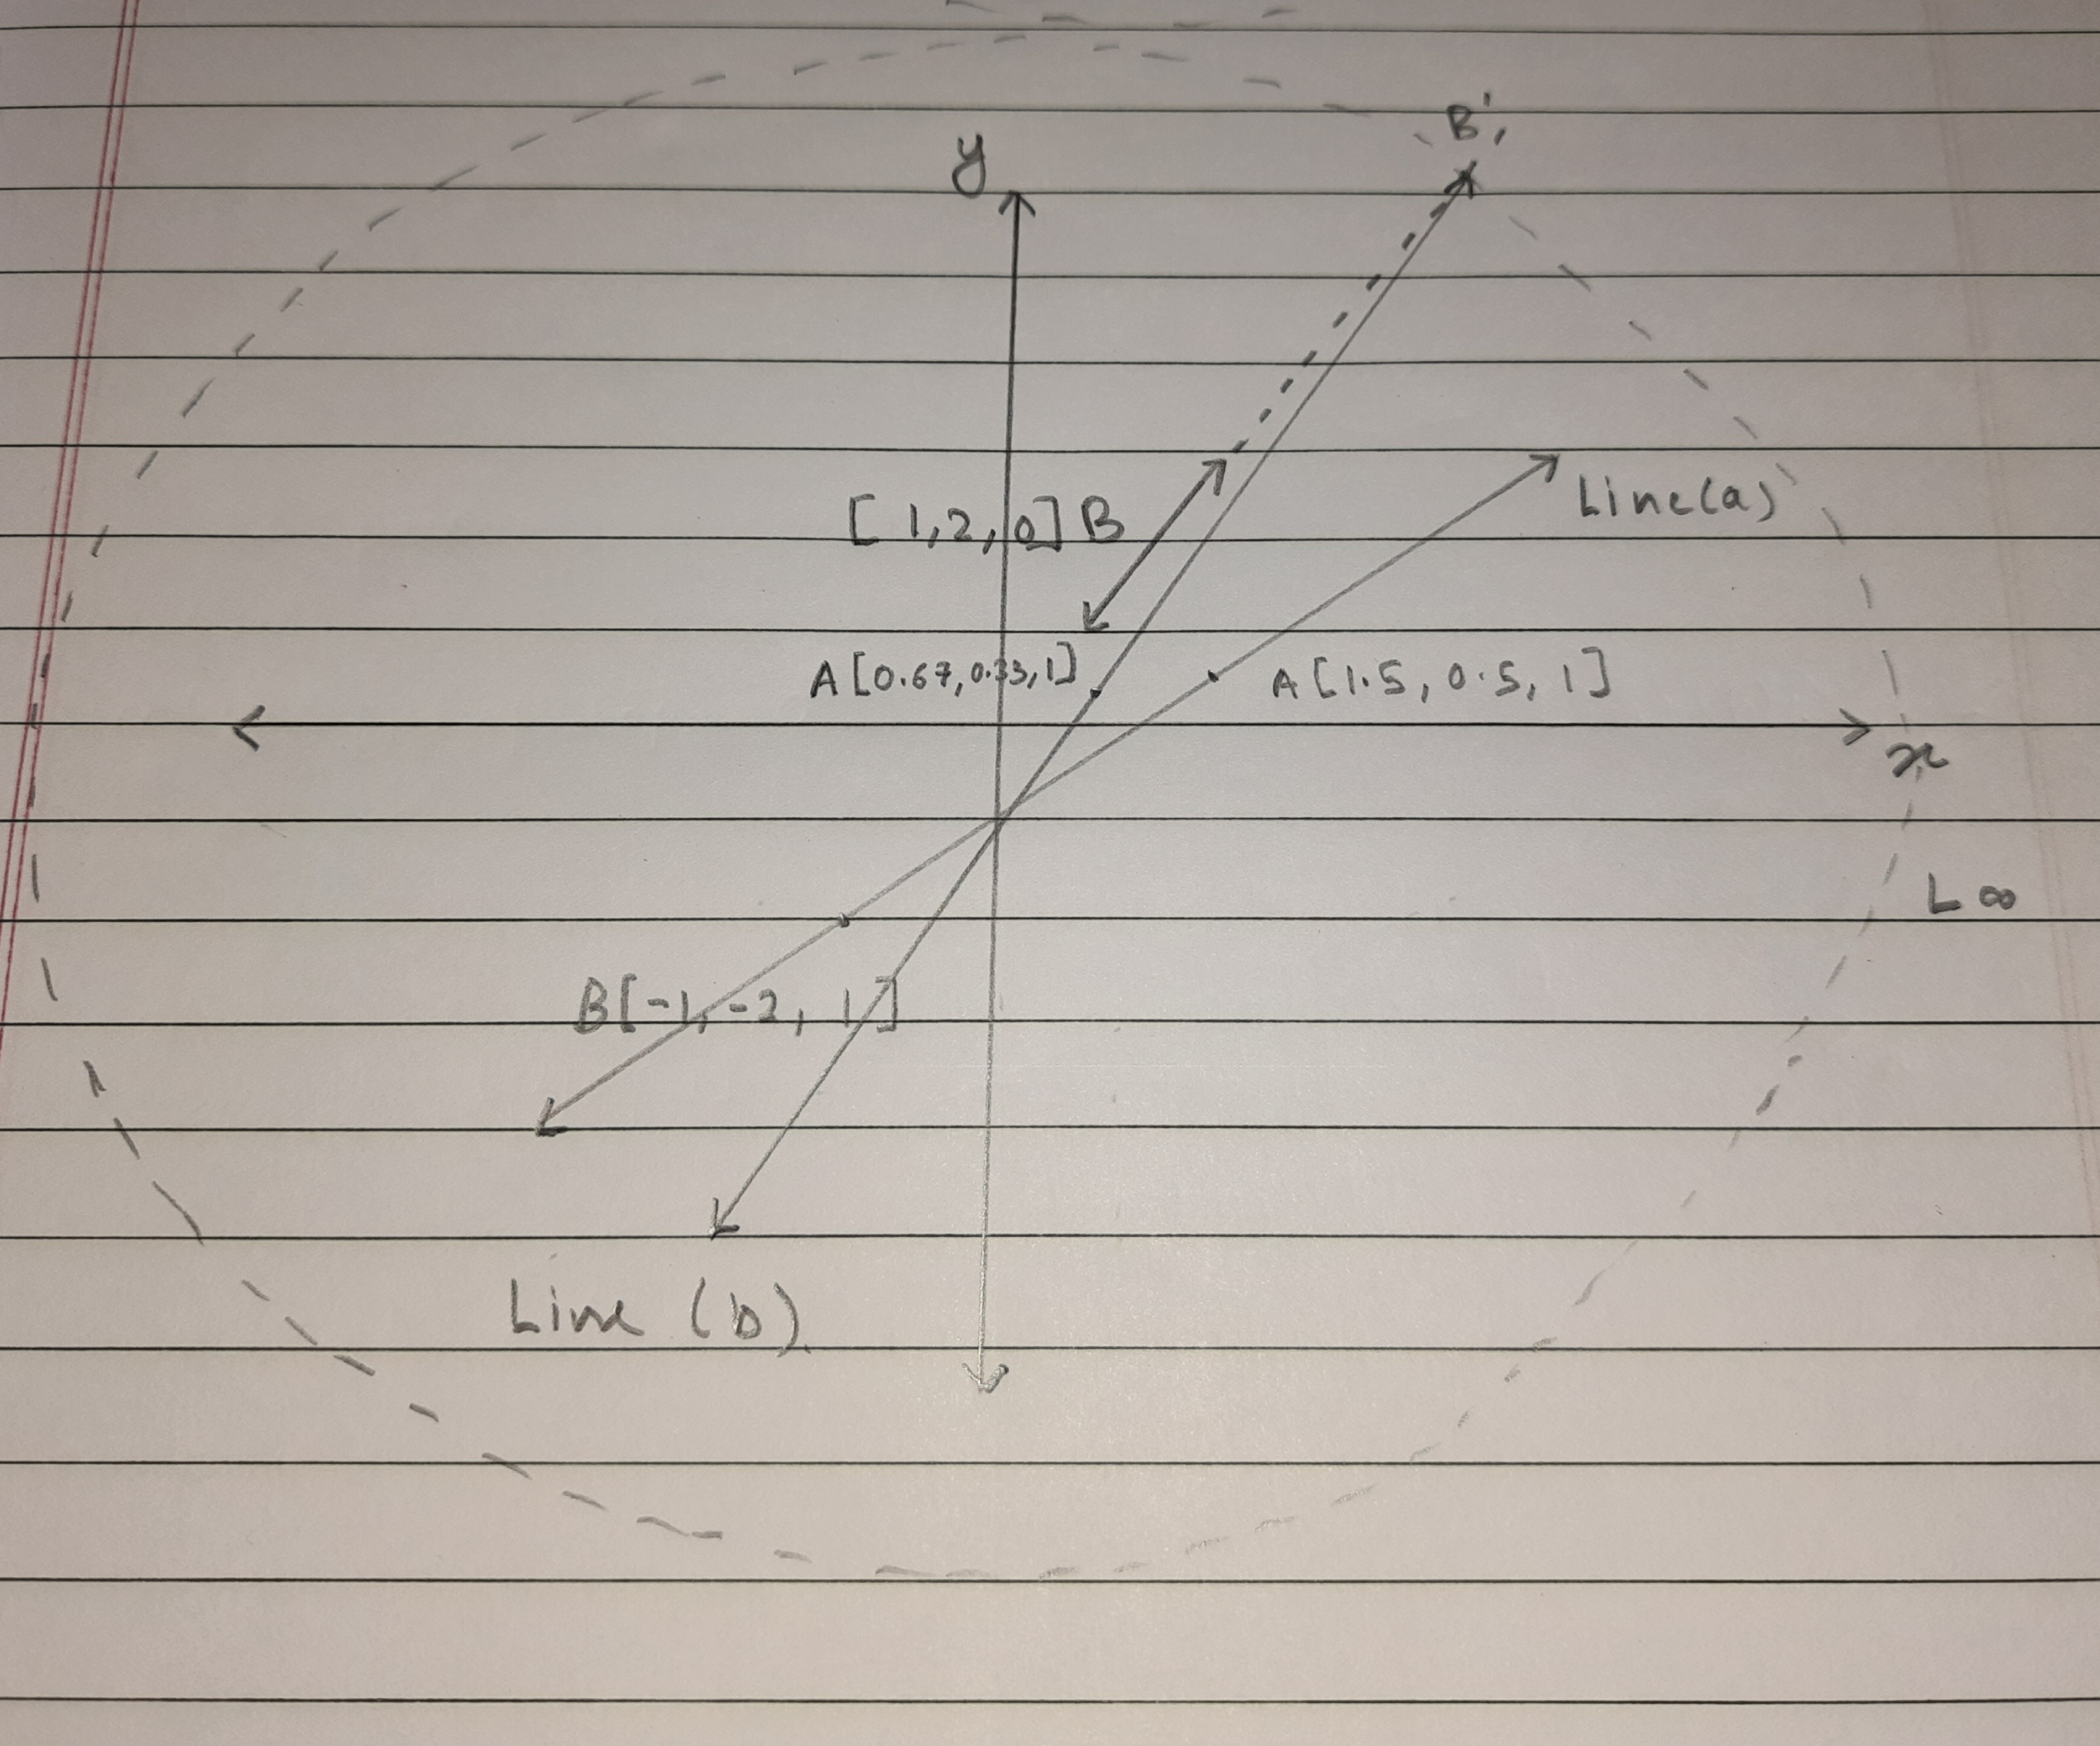
\includegraphics[width = \textwidth, height = 8cm]{02.jpg}
    \caption{{\color{blue} Figure showing the line $AB$ for cases (a) and (b)}}
    \label{fig:my_label}
\end{figure}
% \vspace{6cm}
\end{studentSpace}
\end{tcolorbox} 

%%%%% Question 8
\begin{tcolorbox}
\item  Find the standard homogeneous coordinates of the point of
  intersection for each pair of lines. 
\begin{multicols}{2}
\begin{enumerate}[]
\item
$p_1 + p_2 - 2p_3 = 0, 3p_1 + p_2 + 4p_3 = 0$
\item
$p_1 + p_2 = 0, 4p_1 - 2p_2 + p_3 = 0$
\end{enumerate}
\end{multicols}
\begin{studentSpace}
% \vspace{3cm}
{\color{blue}
The homogenous coordinate of the point of intersection of two lines can be found through the cross product of their vector representations in $P^{2}$.\\

a) $L1:[1,1,-2]$ and $L2:[3,1,4]$\\
Points of intersection : $L1 \times L2$ \Rightarrow $[1,1,-2] \times [3,1,4]$ = $[6,-10,-2]$ which is equivalent to $[3,-5,-1]$\\

a) $L1:[1,1,0]$ and $L2:[4,-2,1]$\\
Points of intersection : $L1 \times L2$ \Rightarrow $[1,1,0] \times [4,-2,1]$ = $[1,-1,-6]$\\
}
\end{studentSpace}
\end{tcolorbox}

%%%%% Question 9
\begin{tcolorbox}
\item  Determine which of the following sets of three points are collinear. 
\begin{multicols}{2}
\begin{enumerate}[]
\item
$A[1,2,1]$, $B[0,1,3]$, $[2,1,1]$
\item
$A[1,2,3]$, $B[2,4,3]$, $[1,2,-2]$
\end{enumerate}
\end{multicols}
\begin{studentSpace}
% \vspace{6cm}
{\color{blue}
For collinear points, the pairwise cross product of their homogeneous coordinates should result in the same line. Moreover, the determinant of the three vectors should be zero.\\

a) $A \times B \times C \Rightarrow det(A,B,C) = 1(-2) -2(-6) + 1(-2) = 8$, since $det(A,B,C) \neq 0$, thus points are not collinear.\\

b) $A \times B \times C \Rightarrow det(A,B,C) = 1(-14) -2(-7) + 3(0) = 0$, since $det(A,B,C) = 0$, thus points are collinear.\\
}
\end{studentSpace}
\end{tcolorbox} 

%%%% Question 10
\begin{tcolorbox}
\item  Determine which of the following sets of three lines meet in a
  point. 
\begin{multicols}{2}
\begin{enumerate}[]
\item
$l[1,0,1], m[1,1,0], n[0,1,-1]$
\item
$l[1,0,-1], m[1,-2,1], n[3,-2,-1]$
\end{enumerate}
\end{multicols}
\begin{studentSpace}
{\color{blue}
We know that by taking cross product of the homogeneous coordinates of two points in $P^{2}$ we get the vector coordinates of the line between them. Similarly, if we take the cross product between two line vectors in $P^{2}$, we can get their point of intersection. Now, to check if there if three points intersect at a single point, the corresponding determinant of the homogeneous coordinates of the three point should be 0.\\

a) $det(l,m,n) = 1(-1) -0(-1) + 1(1) = 0$, thus the lines meet at a point.\\
b) $det(l,m,n) = 1(4) -0(-4) + -1(-2 + 6) = 0$, the lines meet at a point.

}
% \vspace{6cm}
\end{studentSpace}
\end{tcolorbox}

\end{enumerate}
\end{document}

